\documentclass{report}
 
\usepackage[utf8]{inputenc} 
\usepackage[T1]{fontenc}      
\usepackage[top=3.5cm, bottom=3cm, left=3.0cm, right=3.0cm]{geometry}
\usepackage{graphicx}
\usepackage{amsmath}
\graphicspath{{figures/}{../figures}}

\begin{document}

\section*{Questions de cours}
\begin{itemize}

	\item[•] Énoncez les formes canoniques des filtres passe-bas, passe-haut et passe bande d'ordre 2. Pour ce dernier, tracez le diagramme de Bode en fonction des différentes paramètres.
	
	\item[•] Quelles sont les caractéristiques d'un AO idéal ?

	\item[•] Donnez le schéma de montage d'un \textbf{amplificateur non inverseur} en précisant la fonction de transfert.
	
	\item[•] Qu'est-ce qu'un circuit stable ? Quel est le critère de stabilité pour un quadripôle d'ordre 2 en régime libre (c'est-à-dire quand on branche la sortie sur l'entrée) ?

\end{itemize}

\section*{Exercices supplémentaires (difficile)}

\begin{itemize}

	\item[•] Comment réaliser une source de courant parfaite ?
	
	\item[•] Dans un montage amplificateur non-inverseur, comment minimiser la puissance dissipée par l'amplificateur opérationnel ?

\end{itemize}

\newpage

\section*{Puissance consommée par un AO $\bullet\circ\circ$}
 
On souhaite alimenter un dispositif électrique (en rouge) modélisé par une résistance de charge $R_c$ avec une tension nominale $V_{nom}$. On dispose pour cela d'une source de tension (en bleue) mais dont la tension de sortie maximale $V_{max}$ est $V_{max} = V_{nom}/2$, insuffisante pour l'usage voulu. On introduit un montage intermédiaire pour compenser l'insuffisance de la source. 

\begin{figure}[!h]
\centering
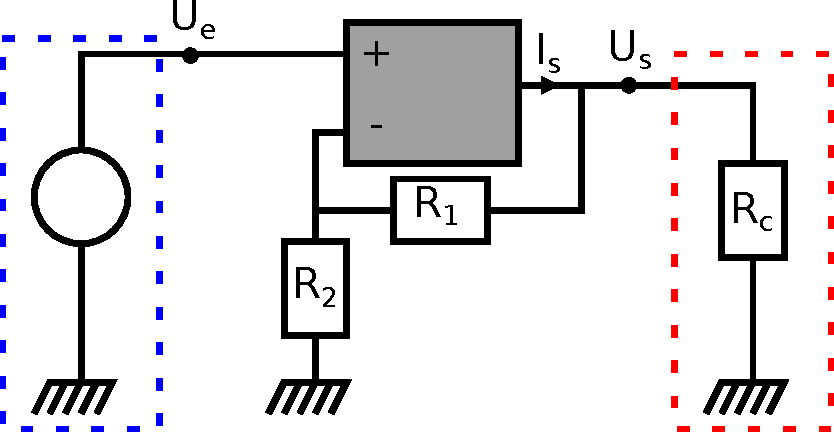
\includegraphics[width=0.5\linewidth]{puissance_AO.pdf}
\end{figure}

\begin{itemize}
	\item[•] Calculer $U_s$ en fonction de $U_e$ et déterminer le rôle de ce montage. Comment doit-on choisir $R_1$ et $R_2$ pour que $U_s = V_{nom}=2V_{max}$ ?
	\item[•]  On suppose dans un premier temps que $R_c=\infty$, cad que la résistance de charge n'est pas connectée au circuit. Quelle est la puissance électrique émise par l'AO ?
	\item[•] On suppose maintenant que le circuit est connecté à la charge, cad que $R_c$ est finie. Quelle est désormais la puissance dégagée par l'AO ?
	\item[•] Comment choisir $R_1$ et $R_2$ de sorte à minimiser la puissance sortie par l'AO ?
\end{itemize}

\newpage

\section*{\textit{Correction Puissance consommée par un AO}}

\begin{itemize}
	\item[•] Amplificateur non-inverseur $u_s = \frac{R_1+R_2}{R_2}u_e$. Pour que $U_s = V_{nom}=2V_{max}$ il faut que le montage double la tension, cad $R_1=R_2$.
	\item[•]  Si $R_c=\infty$, alors le courant dans la charge $i_c$ est nul. Alors $P=u_si_s= \frac{R_1+R_2}{R_2^2}u_e^2$. L'AO consomme de l'énergie même s'il n'y a aucune puissance délivrée à la charge !
	\item[•] Soit $i_1$ le courant traversant $R_1$ et $R_2$. Alors la loi des nœuds donne : $i_s-i_1-ic=0$ (signe pris tq les puissances soient positives). On a alors :
	\begin{equation}
		P=u_si_s=\frac{R_1+R_2}{R_2^2}u_e^2+\frac{(R_1+R_2)^2}{R_2^2R_c}u_e^2
	\end{equation}
	\item[•] On prend $R_2\gg R_c$, le premier terme de dissipation de l'AO devient négligeable devant la puissance envoyée à la charge.
\end{itemize}

\newpage

\section*{Montage passe-bas $\bullet\bullet\circ$}

On considère le montage suivant. L'AO est supposé idéal.

\begin{figure}[!h]
\centering
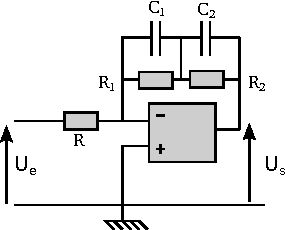
\includegraphics[width=0.5\linewidth]{circuit_6.pdf}
\end{figure}

\begin{itemize}

	\item[$\ast$] Montrer que la fonctiond e transfert de ce filtre s'écrit sous la forme :
\begin{equation}
	H=H_0\frac{1+j\omega/\omega_0}{(1+j\omega/\omega_1)(1+j\omega/\omega_2)}
\end{equation}
On donnera l'expression de $\omega_0$, $\omega_1$ et $\omega_2$.

\item[$\ast$] Tracer le diagramme de Bode correspondant en fonction des différentes pulsations en jeu. Expliciter les cas possibles.

\item[$\ast$] On considère désormais que $R=R_1=R_2$ et $C_1=C_2=C$. Simplifier la fonction de transfert, en introduisant $\omega_0=1/RC$. A quel type de filtre à t-on affaire ?

\item[$\ast$] On envoie en entrée le signal suivant :
\begin{equation}
	U_e(t) = \frac{4U_0}{\pi}\sum_{p=0}^{\infty}\frac{1}{2p+1}\sin(2(p+1)\omega t)
\end{equation}
On suppose que $\omega\gg\omega_0$. Quel est le signal de sortie $U_s$ ? Donner son allure et commenter. 

\end{itemize}

\newpage

\section*{\textit{Correction Montage passe-bas}}

\begin{itemize}

	\item[$\ast$] Fonction de transfert :
\begin{equation}
	H=\frac{u_s}{u_e}=\frac{R_1+R_2}{R}\frac{1+j\frac{R_1R_2}{R_1+R_2}(C_1+C_2)\omega}{(1+jR_1C_1\omega)(1+jR_2C_2\omega)}=H_0\frac{1+j\omega/\omega_0}{(1+j\omega/\omega_1)(1+j\omega/\omega_2)}
\end{equation}
donc $H_0=\frac{R_1+R_2}{R}$, $\omega_0=\frac{R_1+R_2}{R_1R_2(C_1+C_2)}$, $\omega_1=1/R_1C_1$ et $\omega_2=1/R_2C_2$

	\item[$\ast$] Diagramme de Bode : on décompose en somme des diagramme de Bode des différents produits.

\textbf{Cas $\omega_0<\omega_1<\omega_2$ :}
\begin{figure}[!h]
	\centering
	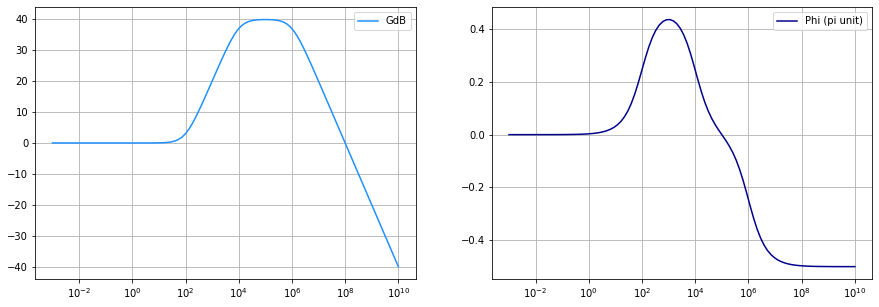
\includegraphics[width=0.8\linewidth]{exo2_0.png}
\end{figure}

\textbf{Cas $\omega_1<\omega_0<\omega_2$ :}
\begin{figure}[!h]
	\centering
	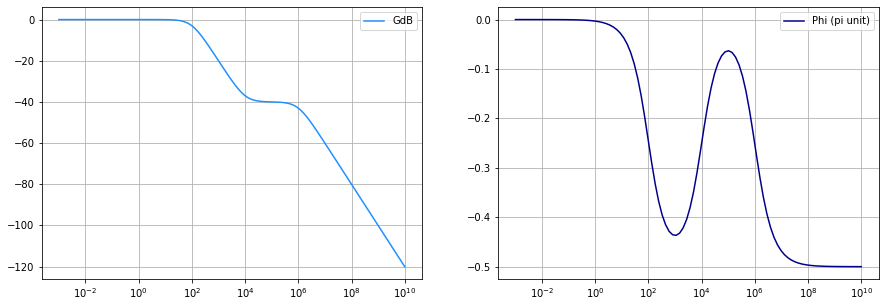
\includegraphics[width=0.8\linewidth]{exo2_1.png}
\end{figure}

\textbf{Cas $\omega_1<\omega_2<\omega_0$ :}
\begin{figure}[!h]
	\centering
	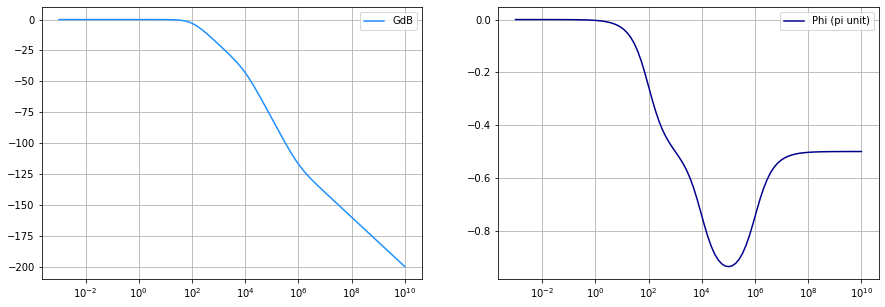
\includegraphics[width=0.8\linewidth]{exo2_2.png}
\end{figure}

	\item[$\ast$] Comme $\omega_0=\omega_1=\omega_2$ et $H_0=2$, la fonction de transfert se simplifie en : 
\begin{equation}
	H=\frac{2}{(1+j\omega/\omega_0)}
\end{equation}	
C'est un filtre passe-bas d'ordre 1.

\item[$\ast$] Le signal d'entrée est un signal créneau (pair, avec les cosinus) : on reconnait la décroissance typique en $1/n$ avec les $n$ impairs seulement. Les coefficients de Fourier sont :

\begin{equation}
	\left\lbrace
	\begin{array}{lll}
		C_n &= \frac{4U_0}{\pi}\frac{1}{2(p+1)}\\
		\varphi_n &= -\frac{\pi}{2} \\
	\end{array}\right.
\end{equation}

On rappelle l'écriture de la décomposition de Fourier :
\begin{equation}
	U_e(t) = \sum_{p=0}^{\infty}C_n\cos(n\omega t+\varphi_n)
\end{equation}

La fonction de transfert, dans le cas où $\omega\gg\omega_0$, peut se simplifier en $H\simeq\frac{2\omega_0}{j\omega}$. Les coefficients de Fourier du signal de sortie sont alors : 

\begin{equation}
	\left\lbrace
	\begin{array}{lll}
		C'_n & = \frac{4U_0}{\pi}\frac{1}{2(p+1)}\times |H(2(p+1)\omega)|\\

		\varphi_n' &= -\frac{\pi}{2}+\mathbf{arg}\left(\frac{2\omega_0}{j\omega} \right)  \\
	\end{array}\right.
\end{equation}

On obtient donc :
\begin{equation}
	\left\lbrace
	\begin{array}{lll}
		C'_n & = \frac{4U_0}{\pi}\frac{2}{(2(p+1))^2}\frac{\omega_0}{\omega}\\
		\varphi_n' &= -\frac{\pi}{2}-\frac{\pi}{2} \\
	\end{array}\right.
\end{equation}

Le signal de sortie est donc :

\begin{equation}
	U_s(t) = \frac{2U_0}{\pi}\sum_{p=0}^{\infty}\frac{1}{(2p+1)^2}\cos(2(p+1)\omega t -\pi)
\end{equation}

On reconnait la décroissance en $1/n^2$ typique d'un signal triangulaire. C'est normal : le filtre se comporte ici comme un intégrateur.

\end{itemize}

 \newpage

\section*{Exercice 3 $\bullet\bullet\bullet$}

On considère le filtre suivant :

\begin{figure}[!h]
\centering
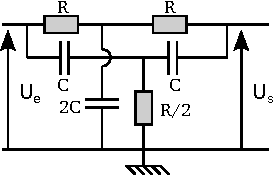
\includegraphics[width=0.5\linewidth]{circuit_2.pdf}
\end{figure}

\begin{itemize}

	\item[$\spadesuit$] Quel est le comportement de ce filtre à basse et haute fréquence ? 
	
	\item[$\spadesuit$] Montrer que la fonction de transfert peut s'écrire sous la forme :
	\begin{equation}
		H(x) =\frac{1+(jx)^2}{1+4jx + (jx)^2}
	\end{equation}
	où $x=\omega/\omega_0$ avec $\omega_0$ une pulsation que l'on déterminera. Tracer le diagramme de Bode correspondant. 
	
	\item[$\spadesuit$] Déterminer la bande "coupante" $\Delta\omega$, cad la plage de pulsations $\Delta\omega$ pour lesquelles $G^{dB}(\omega)\leq G^{dB}_{max} - 3$. On rappelle que $20\log\left( \sqrt{2}\right)\simeq3 $.
	
	\item[$\spadesuit$] On envoie le signal $U_e(t)=U_0\cos^3(\omega t)$ en entrée, avec $\omega=\omega_0/3$. Déterminer le signal de sortie $U_s(t)$. Tracer schématiquement les signaux.

\end{itemize}

\newpage

\section*{\textit{Correction exercice 3}}

Le courant de sortie est supposé nul.

\begin{itemize}
	\item[$\spadesuit$] Comportement : BF, $u_e=u_s$ et HF, $u_e=u_s$, c'est un filtre coupe-bande (l'inverse d'un passe-bande, qui ne laisse rien passer à BF et HF). En BF, le circuit est "flottant", cad il n'es tplus connecté à la masse. Comme l'intensité de sortie est considérée comme nulle, la chute de tension aux bornes des résistances est nulle.
	
	\item[$\spadesuit$]
		Pour la fonction de transfert, on fait une loi des nœuds en A (entre les 2 résistances du haut), en B (entre les 2 capa du milieu) et à la sortie :
		
\begin{equation}
	\left\lbrace
	\begin{array}{lll}
		 \frac{u_e-u_A}{R} + \frac{u_s-u_A}{R} -2jC\omega u_A = 0\\
		 \\
		 jC\omega(u_e-u_B) +  jC\omega(u_s-u_B) - \frac{2}{R}u_B =0  \\
		 \\
		 \frac{u_A-u_s}{R} + jC\omega(u_B-u_s)=0
	\end{array}\right.
\end{equation}

Avec les deux premières lignes, on trouve :

\begin{equation}
	\left\lbrace
	\begin{array}{lll}
		 u_A = \frac{u_e+u_s}{2(1+jRC\omega)}\\
		 \\
		 u_B = \frac{u_e+u_s}{2(1+1/jRC\omega)} \\
	\end{array}\right.
\end{equation}

	On trouve alors en réinjectant dans la dernière équation :
	\begin{equation}
		H =\frac{1+(jRC\omega)^2}{1+4jRC\omega + (jRC\omega)^2}
	\end{equation}
	
	Diagramme de Bode :
Diagramme assymptotique :  $\forall \omega, H=0$ et pour $\omega=\omega_0=1/RC$, dirac à "l'envers" avec $H=-\infty$. C'est bien un coupe-bande.
\begin{figure}[!h]
	\centering
	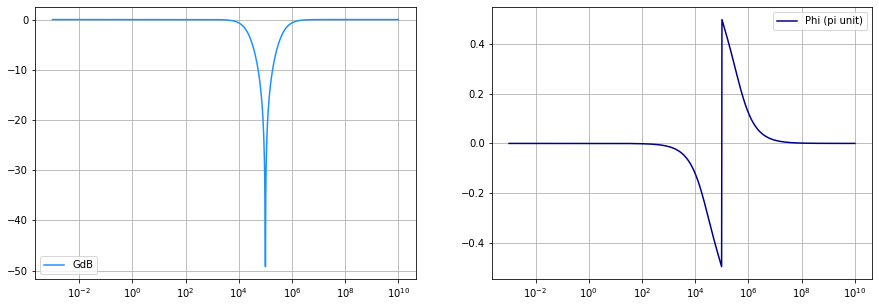
\includegraphics[width=0.8\linewidth]{exo3_0.png}
\end{figure}


	\item[$\spadesuit$] Pour la bande-coupante, on cherche les $\omega$ de telle sorte que :
\begin{equation}
	G_{DB} = -20\log \left( \frac{|1-x^2|}{\sqrt{(1-x^2)^2+16x^2}}\right) = -20\log\left(\frac{1}{\sqrt{2}} \right) \simeq 3
\end{equation}	
	en posant $x=RC\omega$.
On tombe alors sur l'équation $(1-x^2)^2=16x^2$, et en enlevant le carré :
\begin{equation}
	x^2\pm 4x -1 =0
\end{equation}
Avec le signe $\pm$, il y a 4 solutions possibles (2 par équations, qui ont 2 solutions chacunes). Les seules solutions positives sont $\omega_{\pm}=\frac{\pm 2+\sqrt{5}}{RC}$.

	\item[$\spadesuit$] On peut montrer facilement que le signal d'entrée peut s'écrire sous la forme :
	\begin{equation}
		U_e(t)=\frac{1}{4}\left( 3\cos(\omega t) + \cos(3\omega t)\right) 
	\end{equation}
	
	On a donc deux harmoniques, à $\omega$ et $3\omega$, soit :

\begin{equation}
	\left\lbrace
	\begin{array}{lll}
		C_1 & = \frac{3}{4}, \quad \varphi_1=0 \\

		C_3 & = \frac{1}{4}, \quad \varphi_3=0  \\
	\end{array}\right.
\end{equation}	

Ces harmoniques deviennent après sortie du filtre : 
\begin{equation}
	\left\lbrace
	\begin{array}{lll}
		C_1 & = \frac{3}{4}\times |H(\omega)|, \quad \varphi_1=0 + \mathbf{arg}\left(H(\omega) \right)  \\

		C_3 & = \frac{1}{4}\times |H(3\omega)|, \quad \varphi_3=0 + \mathbf{arg}\left(H(3\omega) \right)  \\
	\end{array}\right.
\end{equation}		

Comme $|H(3\omega)| = |H(\omega_0)| = 0$, l'harmonique 3 n'a aucune contribution. Dès lors, pur la première harmonique $x=\omega/\omega_0=1/3$ : 
\begin{equation}
	\left\lbrace
	\begin{array}{lll}
		C_1 & = \frac{3}{4}\times \left|\frac{1-\frac{1}{9}}{1+j\frac{4}{3}-\frac{1}{9}} \right| =\frac{4}{\sqrt{52}} \simeq\frac{1}{2} \\

		\varphi_1 & = -\mathbf{arg}\left( 1+j\frac{4}{3}-\frac{1}{9}\right) =\arctan\left( \frac{27}{32}\right) \simeq \frac{\pi}{4} \\
	\end{array}\right.
\end{equation}		
	
En très grosse approximation, on peut donc dire que :
\begin{equation}
	U_s(t) \simeq \frac{1}{2}\cos(\omega t + \pi/4)
\end{equation}	

\begin{figure}[!h]
\centering
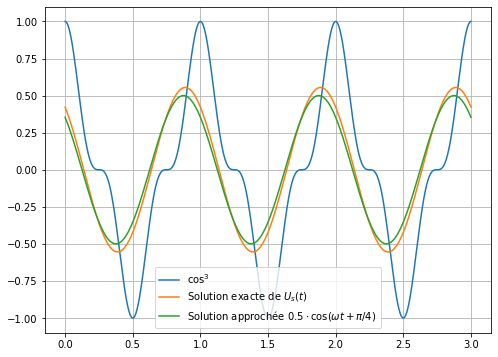
\includegraphics[width=0.5\linewidth]{exo3_1.png}
\end{figure}
	
\end{itemize}

\newpage

\section*{Exercice 4 $\bullet\bullet\circ$}

\begin{itemize}
\item[$\star$] Explicitez la fonction de transfert de ce filtre, puis calculez son gain et sa phase. On notera $\omega_0$ sa pulsation caractéristique. Quel est son rôle ?
\begin{figure}[!h]
\centering
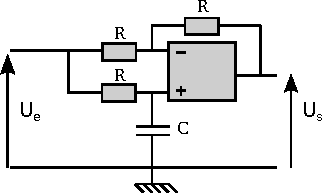
\includegraphics[width=0.5\linewidth]{circuit_.pdf}
\end{figure}

\item[$\star$]
Pour quelles conditions sur le circuit et le signal d'entrée trouve t-on que le circuit retarde un signal périodique sans le déformer, c'est-à-dire que $U_{s}(t)=U_{e}(t-\tau)$ ? Exprimez alors ce retard $\tau$ en fonction de $R$ et $C$.

On pourra utiliser la décomposition en série de Fourier du signal d'entrée :
\begin{equation}
U_e(t) = \sum_n C_n\cos(n\omega t + \varphi_n)
\end{equation}

\item[$\star$] On envoie en entrée le signal suivant :
\begin{equation}
U_{e}(t) = U_{0}\cos^{3}(\omega t)
\end{equation}

Décrire l'effet du filtre sur ce signal pour $\omega = \frac{\omega_{0}}{3}$ et $\omega=10^{-2}\omega_0$, et donner l'allure du signal de sortie. On donne $\arctan(1/3)\simeq\pi/10$.

\item[$\star$]
On suppose le condensateur déchargé à $t=0$. On envoie un échelon de tension $E$ en entrée. Quelle est la sortie ? Commenter.
\end{itemize}

\newpage

\section*{Exercice 4 (MP) $\bullet\bullet\circ$}

On considère le filtre ci-dessous, où l'amplificateur opérationnel (AO) est supposé fonctionner en régime linéaire. On rappelle qu'en régime linéaire, l'AO idéal suit les propriétés suivantes :
\begin{itemize}
	\item[-] les tensions d'entrées sont égales $u_+=u_-$ ;
	\item[-] les courants d'entrées sont nuls $i_+=i_-=0$ ;
\end{itemize}
L'AO ajuste à tout instant la tension $u_s$ et l'intensité $i_s$ de sortie pour que ces deux conditions soient en permanence vérifiées.

\begin{figure}[!h]
\centering
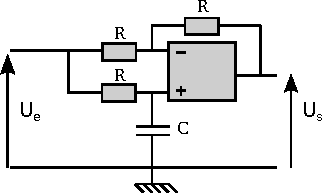
\includegraphics[width=0.5\linewidth]{circuit_.pdf}
\end{figure}

\begin{itemize}
\item[$\star$] Explicitez la fonction de transfert de ce filtre, puis calculez son gain et sa phase. On notera $\omega_0$ sa pulsation caractéristique. Quel est son rôle ?

\item[$\star$]
Pour quelles conditions sur le circuit et le signal d'entrée trouve t-on que le circuit retarde un signal périodique sans le déformer, c'est-à-dire que $U_{s}(t)=U_{e}(t-\tau)$ ? Exprimez alors ce retard $\tau$ en fonction de $R$ et $C$.

On pourra utiliser la décomposition en série de Fourier du signal d'entrée :
\begin{equation}
U_e(t) = \sum_n C_n\cos(n\omega t + \varphi_n)
\end{equation}

\item[$\star$] On envoie en entrée le signal suivant :
\begin{equation}
U_{e}(t) = U_{0}\cos^{3}(\omega t)
\end{equation}

Décrire l'effet du filtre sur ce signal pour $\omega = \frac{\omega_{0}}{3}$ et $\omega=10^{-2}\omega_0$, et donner l'allure du signal de sortie. On donne $\arctan(1/3)\simeq\pi/10$.

\item[$\star$]
On suppose le condensateur déchargé à $t=0$. On envoie un échelon de tension $E$ en entrée. Quelle est la sortie ? Commenter.
\end{itemize}

\newpage

\section*{\textit{Correction exercice 4}}

\begin{itemize}
	\item[$\star$]
	$H=\frac{1-jRC\omega}{1+jRC\omega}$. On remarque que $\mid H\mid=1$, mais que $\varphi=-2\arctan(RC\omega)=-2\arctan(\omega/\omega_0)$, avec $\omega_0=1/RC$. On peut écrire alors $H$ sous la forme :
	\begin{equation}
		H=e^{-2j\arctan(RC\omega)}
	\end{equation}
C'est un filtre déphaseur.

	\item[$\star$]
	On part de la décomposition de Fourier d'un signal (quelconque) d'entrée :
\begin{equation}
	U_e(t) = \sum_n C_n\cos(n\omega t + \varphi_n)
\end{equation}	
Après le passage dans le filtre, le signal de sortie :	
\begin{equation}
	\begin{array}{lll}
		U_s(t) & = \sum_n C_n|H(n\omega)|\cos(n\omega t + \varphi_n + \mathbf{arg}(H(n\omega)) \\

		 & = \sum_n C_n\cos(n\omega t + \varphi_n -2\arctan(RCn\omega)) \\
	\end{array}
\end{equation}			
	Or, pour obtenir une forme retardée comme proposée dans l'énoncé, il faut factoriser par le $n\omega$ compris dans le $\arctan$. On le linéarise dans le cas où $RCn\omega\ll1$, cad $\omega\ll\omega_0$ avec $1/\tau=1/2RC$. 
	
	Dans ce cas-là :
\begin{equation}
	\begin{array}{lll}
		U_s(t) & = \sum_n C_n\cos(n\omega t + \varphi_n -2RCn\omega) \\

		 & = \sum_n C_n\cos(n\omega (t-\tau) + \varphi_n) \\
		 &= U_e(t-\tau)
	\end{array}
\end{equation}			
	Il faut donc que $\omega\ll 1/RC$, avec toutes les harmoniques qui valident cette condition (ex : signal triangulaire, avec une décroissance rapide de l'amplitude des harmoniques).
	
	\item[$\star$] On décompose le signal en une série de cosinus : $\cos^3(\omega t)=\frac{1}{4}(3\cos(\omega t) + \cos(3\omega t))$.
	Le signal de sortie sera donc : 
	\begin{equation}
	U_s(t) = \frac{1}{4}\left[ 3\cos(\omega t - 2\arctan(\omega/\omega_0)) + \cos(3\omega t - 2\arctan(3\omega/\omega_0))\right] 
	\end{equation}
	Pour $\omega = \frac{\omega_{0}}{3}$, on a :
\begin{equation}
	\begin{array}{lll}
		U_s(t) & = \frac{3}{4}\cos(\omega t - 2\arctan(1/3)) + \frac{1}{3}\cos(3\omega t - 2\arctan(1) \\

		 & \simeq \frac{3}{4}\cos(\omega t - \pi/5) + \frac{1}{3}\cos(3\omega t - \pi/2)\\
	\end{array}
\end{equation}		
	Pour $\omega = 10^{-2}\omega_0$, on a la condition $\omega\ll\omega_0$, avec un retard de phase $\varphi = 2\cdot10^{-2}$.
	
	\item[$\star$] Pour $t<0$, le condensateur est déchargé donc $u_e(t)=u_s(t)=0$. Pour $t\geq0$, le condensateur se charge donc $u_-(t) = E(1-e^{-t/RC})$, et alors :
	\begin{equation}
		u_s(t)=2E(1-e^{-t/RC}) - E
	\end{equation}
	Le signal finit bien par "redevenir" celui d'entrée (car $H=1$) mais un retard. Attention, ici c'est une transformation de Fourier et non une série de Fourier qu'il faut opérer. 
	
\end{itemize}

\newpage

\section*{Exercice 5 $\bullet\circ\circ$}

On considère le montage ci-dessous :
\begin{figure}[!h]
\centering
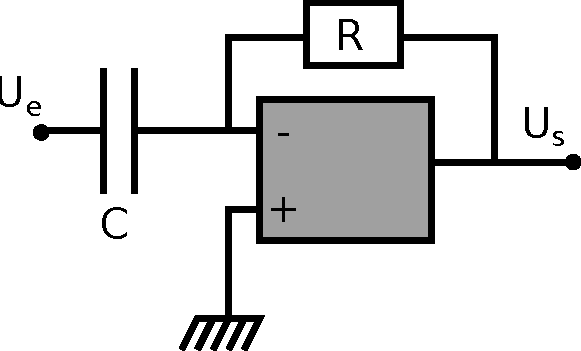
\includegraphics[width=0.5\linewidth]{derivateur.pdf}
\end{figure}
\begin{itemize}
	\item[•] On suppose dans un premier temps que l'AO est idéal. Qu'est-ce que cela signifie ? Calculez la fonction de transfert de ce montage. Quel est son rôle ?
	\item[•] On suppose désormais que l'AO est réel. On suppose alors que la sortie $u_s$ est reliée à $\varepsilon=u_+-u_-$ par la relation :
	\begin{equation}
		\tau\frac{du_s}{dt} +u_s = \mu_0\varepsilon
	\end{equation}
	avec $\mu_0=10^5$ et $\frac{\mu_0}{2\pi\tau}=$1MHz.
	
	Quel est la nouvelle fonction de transfert ? 
	
	Le montage est il stable ?
	
	\item[•] Que se passe t-il si l'on intervertit les bornes + et - de l'AO ?
	
	\item[•] A quel type de montage ce circuit s'apparente t-il ? Calculez ses caractéristiques pour $R=10$k$\Omega$ et $C=$100nF. Pour quelle fréquences agit-il comme un dérivateur ? 
\end{itemize}

\newpage

\subsection*{\textit{Correction exercice 5}}

\begin{itemize}
	\item[•] $H = -jRC\omega$ cad $u_s(t) = -RC\frac{du_e}{dt}$. C'est un dérivateur.
	\item[•] En TF : $u_s = \varepsilon\frac{\mu_0}{1+j\tau\omega}$. Puis loi des nœuds, avec $\varepsilon=u_-$ :
	\begin{equation}
		H(j\omega) = \frac{-\mu_0jRC\omega}{1+\mu_0 + j\omega(\tau+RC)-RC\tau\omega^2}
	\end{equation}
	L'équation différentielle associée à tous ses coefficients du même signe, les solutions sont sinusoïdales donc bornées. 
	\item[•] En inversant les pôles, $\varepsilon=+u_-$. Cela revient à remplacer $\mu_0\leftarrow-\mu_0$. Le terme de dérivée 0 devient alors $1-\mu_0$ et est négatif donc la solution contient une partie exponentielle et diverge jusqu'à saturation.
	\item[•] C'est un filtre passe bande d'ordre 2 de pulsation $\omega_0=\sqrt{\frac{1+\mu_0}{RC\tau}}$
	Sous forme canonique, on a :
		\begin{equation}
		H(j\omega) = \frac{H_0}{1+jQ(x-\frac{1}{x})}
	\end{equation}
	avec $H_0=\frac{\mu_0RC}{\tau+RC}=-5,9\cdot10^3$ et $Q = \frac{\sqrt{(1+\mu_0)RC\tau}}{\tau+RC}=74$
	Ce filtre est dérivateur pour $x$ petit, cad $H\approx \frac{j\omega}{Q\omega_0}$. Cette condition est vérifiée jusqu'à $x\approx0,9$ cad $f=2\pi\omega\approx11$kHz.
\end{itemize}

\newpage

\section*{Exercice 6 (MP)}

On étudie le montage ci-dessous dans lequel l'amplificateur opérationnel est supposé idéal et fonctionner en régime linéaire. On rappelle qu'en régime linéaire, l'AO idéal suit les propriétés suivantes :
\begin{itemize}
	\item[-] les tensions d'entrées sont égales $u_+=u_-$ ;
	\item[-] les courants d'entrées sont nuls $i_+=i_-=0$ ;
\end{itemize}
L'AO ajuste à tout instant la tension $u_s$ et l'intensité $i_s$ de sortie pour que ces deux conditions soient en permanence vérifiées.

\begin{figure}[!h]
\centering
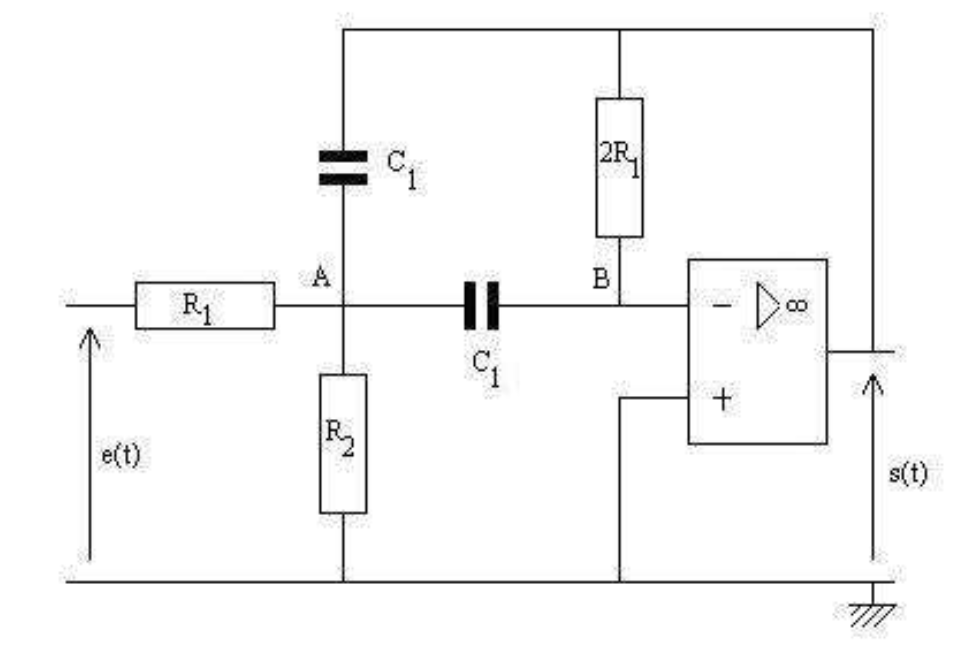
\includegraphics[width=0.5\linewidth]{circuit_12.png}
\end{figure}

\begin{itemize}

	\item[$\star$] Montrer que la fonction de transfert peut se mettre sous la forme canonique :
	\begin{align*}
		H=\frac{H_0}{1+jQ\left(\frac{\omega}{\omega_0}-\frac{\omega_0}{\omega} \right) }
	\end{align*}
Préciser l'expression de $\omega_0$ et de $Q$. 

	\item[$\star$] Etudier les variations du gain (diagramme de Bode) en fonction de la fréquence. Quel est le rôle de ce filtre ?
	
	\item[$\star$] On met en entrée de ce cricuit une fonction créneau $e(t)$ positive de fréquence $f=3$kHz et de valeur maximale $E=10$V. Tracer l'allure du signal de sortie si le circuit est réglé pour $f_0=3$kHz et $Q=20$.
\end{itemize}

\newpage	

\section*{\textit{Correction Exercice 6}}

\begin{itemize}

	\item[$\star$] On applique le théorème de Millman (ou loi des noeuds officiellement...) aux points $A$ et $B$ :
	\begin{align*}
		&\frac{e-V_A}{R_1}-\frac{V_A}{R_2}+jC_1\omega(s-V_A)+jC_1\omega(V_B-V_A)=0 \\
		&\frac{s-V_B}{2R_1}+jC_1\omega( V_A-V_B) = 0
	\end{align*}
	Il faut une troisième équation : on a la condition $V_B=0$. On obtient donc :
	\begin{align*}
		H=\frac{-1}{1+jR_1C_1\omega+\frac{1}{jR_eC_1\omega}}
	\end{align*}
	avec $R_e=\frac{2R_1R_2}{R_1+R_2}$. On trouve donc $Q+\sqrt{R_1/R_e}$ et $\omega=\sqrt{R_1R_e}C_1$.

	\item[$\star$] C'est un passe bande d'ordre 2 de bande passante $\Delta\omega=\omega_0/Q$.
	
	\item[$\star$] Le signal d'entrée a pour coefficients de Fourier : $c_{p+1}=\frac{2E}{(2p+1)\pi}$ avec $p$ entier. Le fondamental vaut $c_0=E/2$. Le circuit étant accordé sur une fréquence de 3kHz avec une bande passante de 0,15kHz, il ne reste que la première harmonique. Le signal en sortie en donc purement sinusoïdal : 
	\begin{align*}
		s(t)=\frac{2E}{\pi}\sin(\omega t)
	\end{align*}
	
\end{itemize}

\newpage

\section*{Rejecteur de bande $\bullet\circ\circ$}

On considère le quadripôle suivant :

\begin{figure}[!h]
\centering
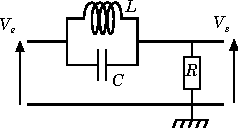
\includegraphics[width=0.5\linewidth]{circuit_12.pdf}
\end{figure}

\begin{itemize}

	\item[$\spadesuit$] Quel est le comportement de ce filtre à basse et haute fréquence ? 
	
	\item[$\spadesuit$] Montrer que la fonction de transfert peut s'écrire sous la forme :
	\begin{align*}
		H(x) =\frac{1+(jx)^2}{1+jQx + (jx)^2}
	\end{align*}
	où $x=\omega/\omega_0$ avec $\omega_0$ et $Q$ une pulsation et un facteur de qualité que l'on déterminera. Tracer le diagramme de Bode correspondant. 
	
	\item[$\spadesuit$] On prend $Q=4$. Déterminer la bande "coupante" $\Delta\omega$, cad la plage de pulsations $\Delta\omega$ pour lesquelles $G^{dB}(\omega)\leq G^{dB}_{max} - 3$. On rappelle que $20\log\left( \sqrt{2}\right)\simeq3 $.
	
	\item[$\spadesuit$] On envoie le signal $U_e(t)=U_0\cos^3(\omega t)$ en entrée, avec $\omega=\omega_0/3$. Déterminer le signal de sortie $U_s(t)$. Tracer schématiquement les signaux.

\end{itemize}

\newpage

\section*{Filtre passif $\bullet\circ\circ$}

On considère le quadripôle suivant :

\begin{figure}[!h]
\centering
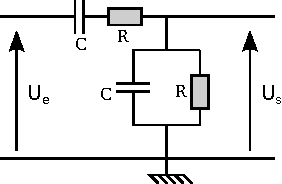
\includegraphics[width=0.5\linewidth]{circuit_1.pdf}
\end{figure}

\begin{itemize}

	\item[$\spadesuit$] Quel est le comportement de ce filtre à basse et haute fréquence ? 
	
	\item[$\spadesuit$] Montrer que la fonction de transfert peut se mettre sous la forme canonique :
	\begin{align*}
		H=\frac{H_0}{1+jQ\left(\frac{\omega}{\omega_0}-\frac{\omega_0}{\omega} \right) }
	\end{align*}
	Tracer le diagramme de Bode correspondant. 
	
	\item[$\spadesuit$] Déterminer la bande passante $\Delta\omega$, cad la plage de pulsations $\Delta\omega$ pour lesquelles $G^{dB}(\omega)\geq G^{dB}_{max} - 3$. On rappelle que $20\log\left( \sqrt{2}\right)\simeq3 $.
	
	\item[$\spadesuit$] On met en entrée de ce circuit une fonction créneau $e(t)$ positive de fréquence $f=3$kHz et de valeur maximale $E=10$V. Tracer l'allure du signal de sortie si le circuit est réglé pour $f_0=3$kHz et $Q=20$.

\end{itemize}


\end{document}
